\chapter{Gyymi}
Neste capítulo é apresentado o projeto do aplicativo Gyymi do ponto de vista do usuário do sistema. Os principais fluxos de uso do aplicativo são expostos, com comentários da parte técnico quando necessários.

% ********
% Cadastro
% ********
\section{Cadastro de Usuários e Estabelecimentos}
Ao entrar acessar o aplicativo pela primeira vez, o usuário encontra a tela de entrada (Figura \ref{fig:landing}). Nesta, três ações podem ser tomadas: cadastrar um estabelecimento (opção "I am a gym"), cadastrar um perfil de treinador (opção "I am a trainer") ou realizar o login na plataforma caso já tenha uma conta (opção "Login to existing account"). A seguir são detalhados os dois fluxos de cadastro do aplicativo.
\begin{figure}[H]
    \centering
    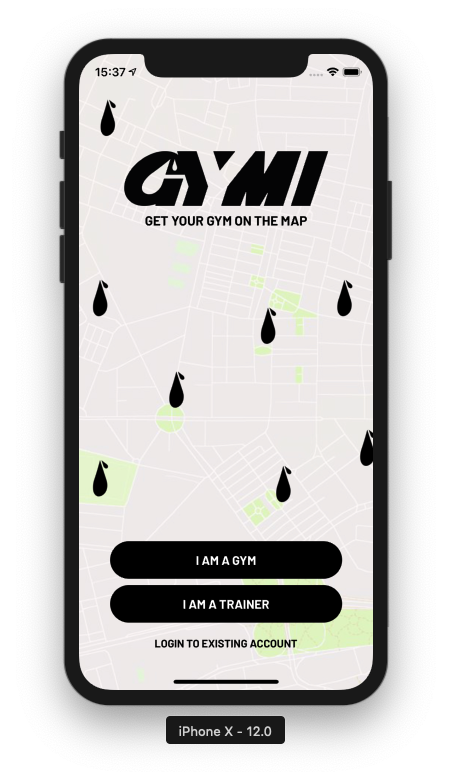
\includegraphics[width=0.4\textwidth]{pfc/figuras/landing.png}
    \caption{Tela de entrada do aplicativo}
    \label{fig:landing}
\end{figure}

% ******************
% Cadastro academias
% ******************
\subsection{Academias} \label{sec:register-gym}
Selecionada a opção por cadastro de um estabelecimento, o usuário primeiramente deve cadastrar os dados do administrador do local (ver Figura \ref{fig:register-manager-data}). Os seguintes dados são solicitados: primeiro nome, último nome, número do celular com código de área, e-mail (com campo de verificação) e senha (com campo de verificação). Para prosseguir com o cadastro, o usuário deve preencher os campos com dados válidos (caso contrário, alertas de erro são apresentados na tela). Ao clicar o botão "Next" uma chamada de API é feita ao back-end passando os dados digitados como parâmetro. Em caso de sucesso, a próxima tela do cadastro é apresentada; em caso de erro (como um e-mail de usuário já cadastrado), um alerta de erro é apresentado - Figura \ref{fig:register-manager-error}.

\begin{figure}[H]
	\centering
    \begin{subfigure}[b]{0.4\textwidth}
        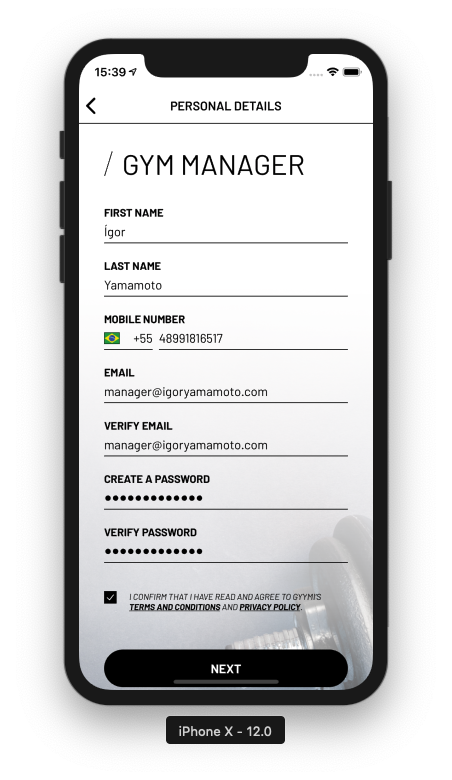
\includegraphics[width=\textwidth]{pfc/figuras/register-manager.png}
        \caption{Dados do administrador}
        \label{fig:register-manager-data}
    \end{subfigure}
    ~
	\begin{subfigure}[b]{0.4\textwidth}
        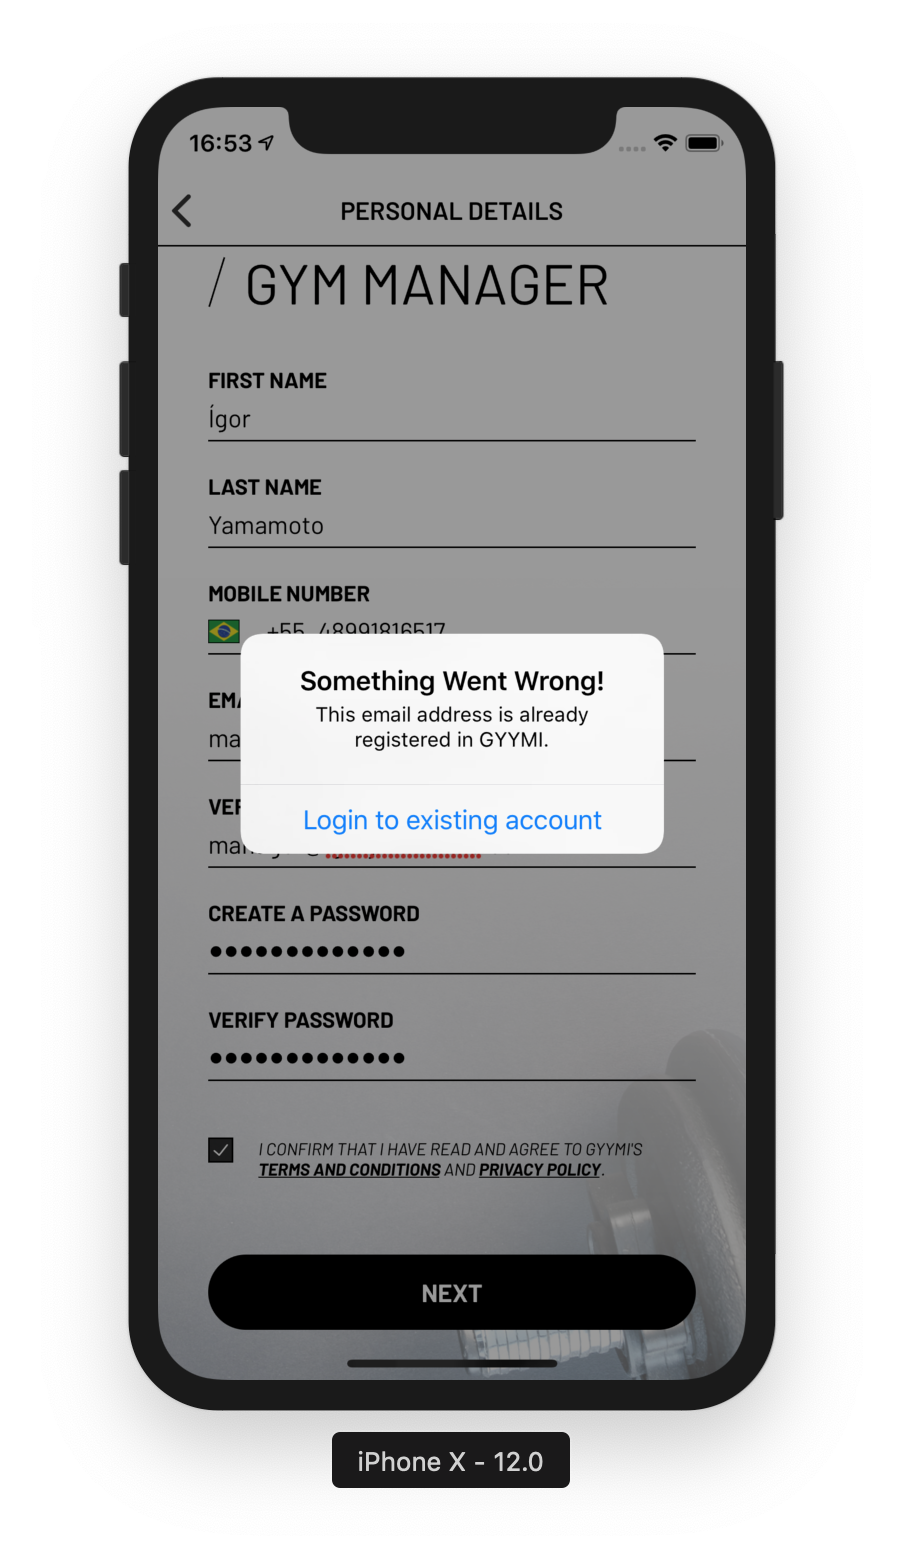
\includegraphics[width=\textwidth]{pfc/figuras/register-manager-error.png}
        \caption{Alerta de erro}
        \label{fig:register-manager-error}
    \end{subfigure}
    ~
    \caption{Tela de cadastro do usuário - administrador da academia}
    \label{fig:register-manager}
\end{figure}

Após o cadastro do usuário administrador da academia ter sido realizado com sucesso, o perfil do estabelecimento é cadastrado. Três telas fazem parte deste fluxo (ver Figura \ref{fig:register-gym}): primeiro informações gerais da academia (nome, endereço, número para contato com o estabelecimento, web-site e endereço de mídias sociais) devem ser passadas - Figura \ref{fig:register-gym-info}; em seguida um tela (Figura \ref{fig:register-gym-amenities}) com opções selecionáveis de facilidades e equipamentos fornecidos pela academia é apresentada; por último, o usuário tem a opção de carregar fotos do estabelecimento (Figura \ref{fig:register-gym-photos}), selecionando uma delas para ser exibida como foto de capa (a ser mostrada no perfil da academia).

\begin{figure}[H]
	\centering
    \begin{subfigure}[b]{0.3\textwidth}
        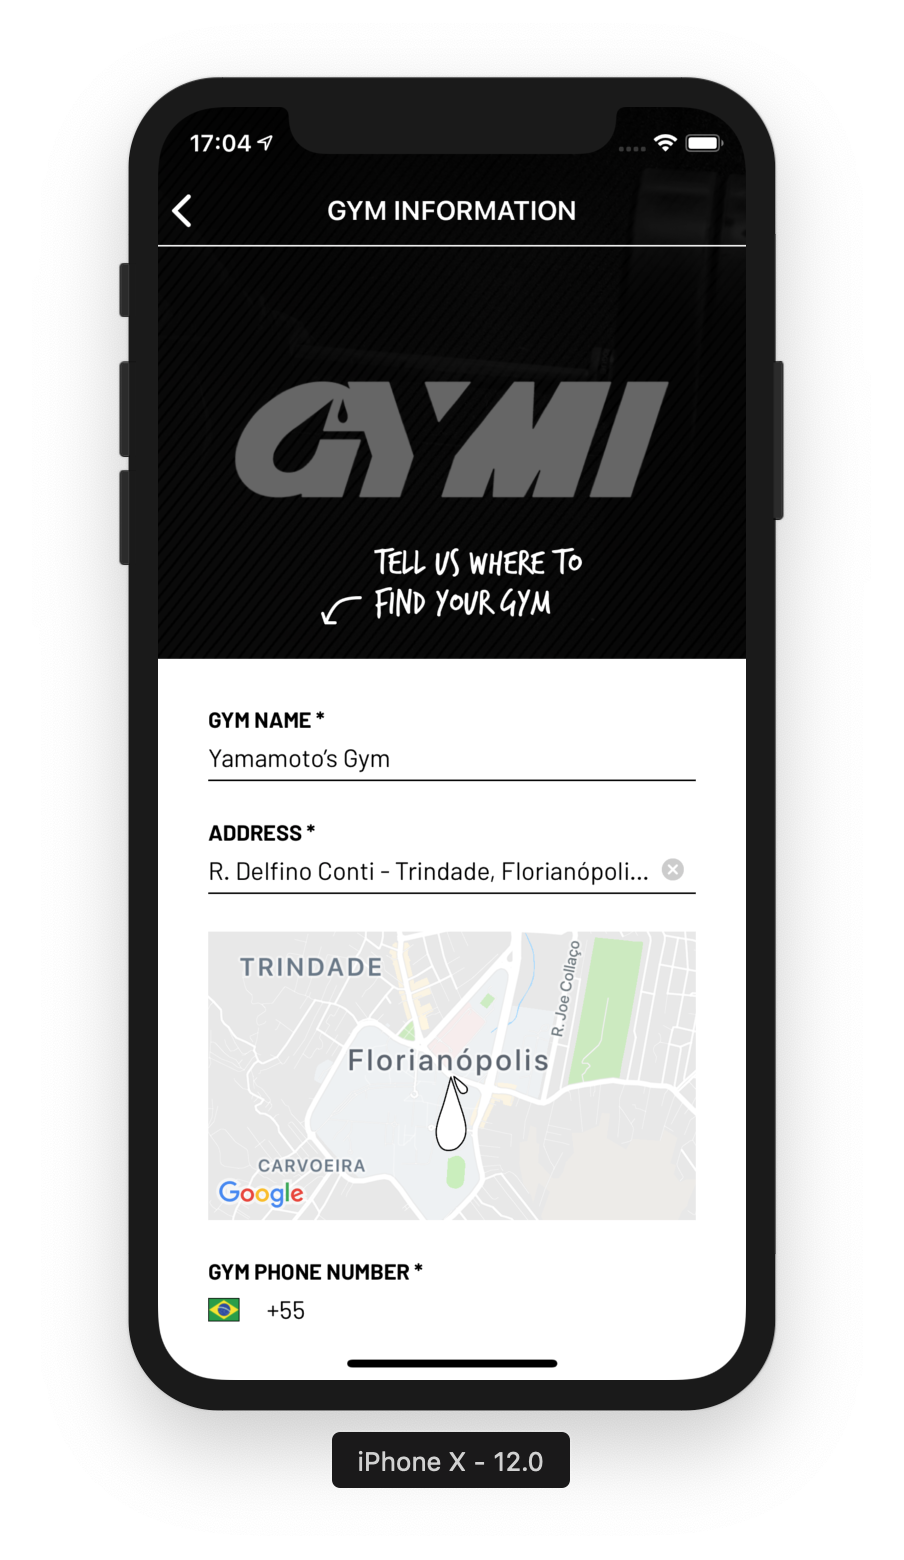
\includegraphics[width=\textwidth]{pfc/figuras/register-gym-info.png}
        \caption{Registro das informações gerais da academia}
        \label{fig:register-gym-info}
    \end{subfigure}
    ~
	\begin{subfigure}[b]{0.3\textwidth}
        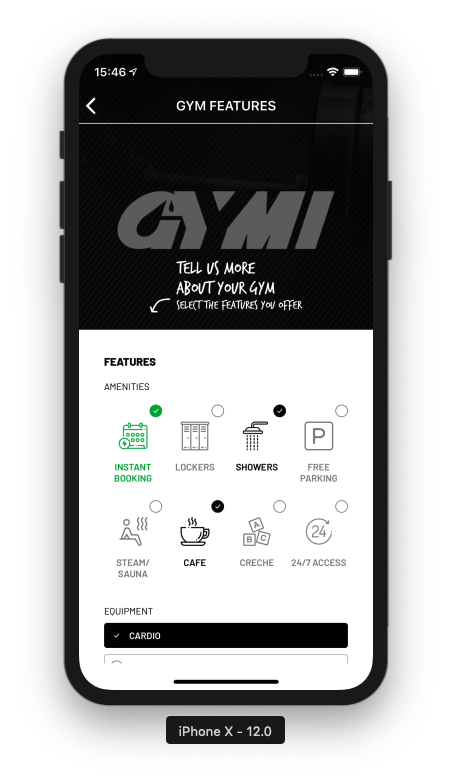
\includegraphics[width=\textwidth]{pfc/figuras/register-gym-amenities.png}
        \caption{Registro das facilidades e equipamentos}
        \label{fig:register-gym-amenities}
    \end{subfigure}
    ~
    \begin{subfigure}[b]{0.3\textwidth}
        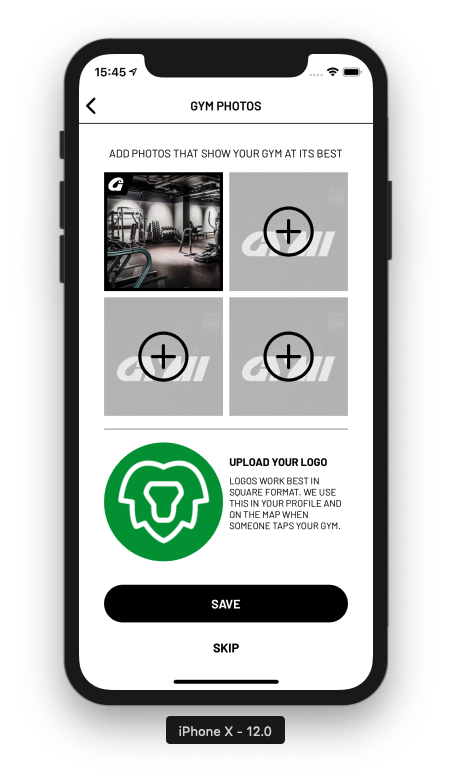
\includegraphics[width=\textwidth]{pfc/figuras/register-gym-photos.png}
        \caption{Registro das fotos do local e da logo}
        \label{fig:register-gym-photos}
    \end{subfigure}
    ~
    \caption{Telas de cadastro de um estabelecimento}
    \label{fig:register-gym}
\end{figure}

Ao término do cadastro do estabelecimento, uma tela de boas vindas (Figura \ref{fig:gym-welcome}) é apresentada ao usuário. A tela apresenta uma marcação (gota de suor branca) da academia em um mapa no local real cadastrado anteriormente (mapa obtido através do serviço do sistema de geolocalização, que é apresentado no próximo capítulo) e outros locais já cadastrados na plataforma são demarcados também (gotas pretas de suor menores), informação proveniente do back-end. A tela apresenta duas opções de ação: registrar detalhes da conta bancária (opção "Add bank details", tela não implementada para a versão piloto do aplicativo) e uma opção para pular o cadastro da conta (opção "Skip"). Ambas as ações levam o usuário as telas de uso da academia, que são apresentadas nas próximas secções.

\begin{figure}[ht]
    \centering
    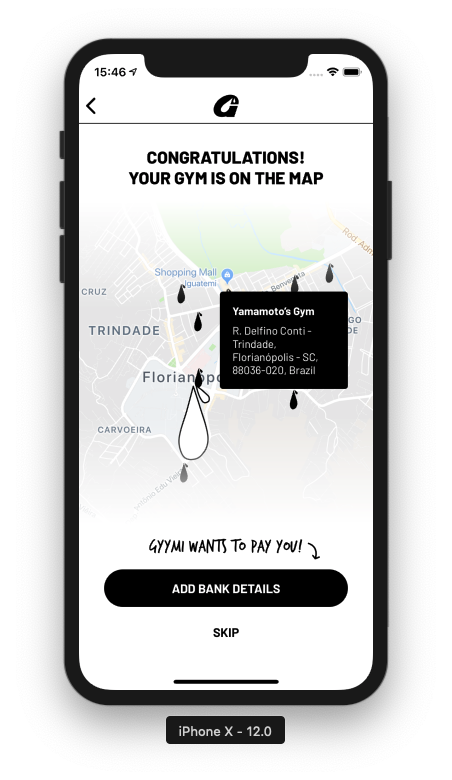
\includegraphics[width=0.4\textwidth]{pfc/figuras/gym-welcome.png}
    \caption{Tela de boas vindas para o estabelecimento}
    \label{fig:gym-welcome}
\end{figure}

% ********************
% Cadastro Treinadores
% ********************
\subsection{Treinadores}
Caso o usuário selecione a opção de cadastro de um treinador na tela de entrada, o mesmo é redirecionado para a tela de cadastro de informações gerais de usuário (Figura \ref{fig:register-trainer-info}), com os seguintes campos de dados: primeiro nome, último nome, e-mail, número do celular, senha (com campo de verificação). Caso as informações preenchidas sejam válidas, o cadastro prossegue para a próxima tela; caso contrário, alertas de erros são exibidos (como no caso do estabelecimento - Secção \ref{sec:register-gym})

Após o preenchimento dos campos, uma requisição para registrar os dados na plataforma é feita para o back-end, o qual faz uma requisição ao serviço de envio de SMS com os dados do número do celular do usuário. Este serviço então envia um SMS com um código de verificação, que deve ser preenchido no campo "Verification Code" da tela de verificação por SMS (ver Figura \ref{fig:register-trainer-verification}). Nesta tela o usuário tem duas opções de ação: verificar o código preenchido (opção que dispara uma nova requisição ao back-end para identificar se o código fornecido é o mesmo gerado pelo serviço de SMS) ou reenviar o código de verificação (opção que desencadeia um novo envio de SMS para o usuário através de nova solicitação para tal ao serviço de SMS).

\begin{figure}[H]
	\centering
    \begin{subfigure}[b]{0.4\textwidth}
        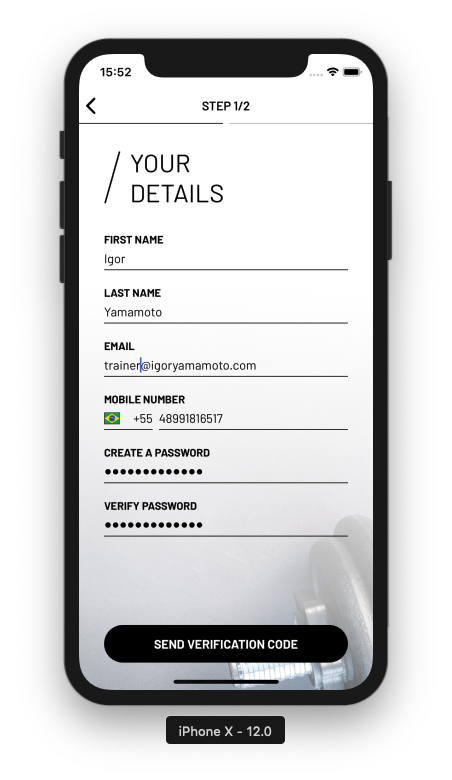
\includegraphics[width=\textwidth]{pfc/figuras/register-trainer.png}
        \caption{Dados do treinador}
        \label{fig:register-trainer-info}
    \end{subfigure}
    ~
	\begin{subfigure}[b]{0.4\textwidth}
        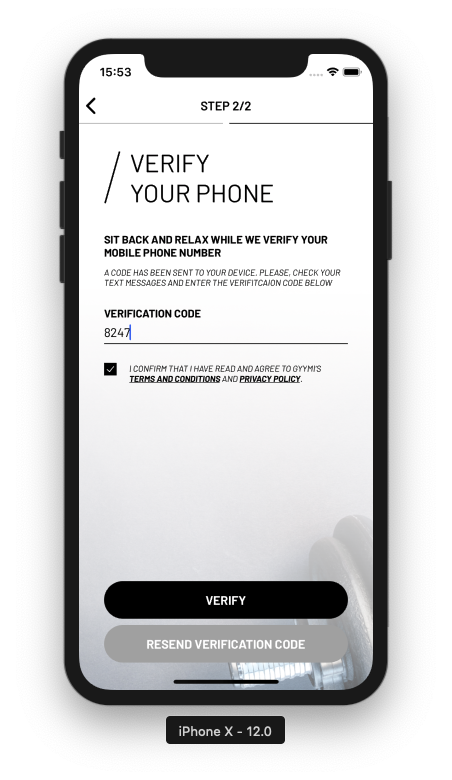
\includegraphics[width=\textwidth]{pfc/figuras/register-trainer-verification.png}
        \caption{Verificação por SMS}
        \label{fig:register-trainer-verification}
    \end{subfigure}
    ~
    \caption{Tela de cadastro do usuário - treinador pessoal}
    \label{fig:register-trainer}
\end{figure}

Uma vez que o código de verificação é validado, o fluxo prossegue para uma tela de boas vindas (Figura \ref{fig:tr-welcome}). Nesta tela, o usuário tem a ação de configurar seu perfil de treinador (opção "Set up your trainer profile") ou a ação de pular esta etapa (opção "Skip"). Caso selecionada a opção de configuração, o cadastro prossegue; caso selecionada a outra opção, o usuário é direcionado a tela principal do treinador.

\begin{figure}[H]
    \centering
    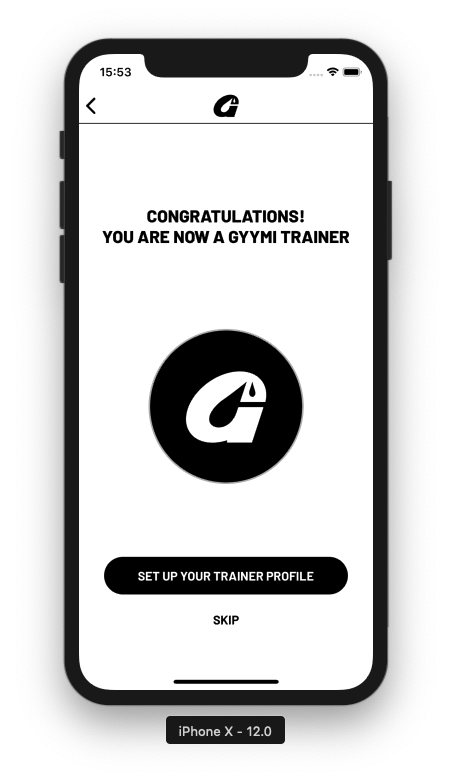
\includegraphics[width=0.4\textwidth]{pfc/figuras/tr-congratulations.png}
    \caption{Tela de boas vindas para o treinador}
    \label{fig:tr-welcome}
\end{figure}

A configuração de perfil de treinador segue um fluxo de três telas (Figura \ref{fig:register-tr-profile}). Primeiro, o usuário deve registrar as informações gerais do perfil (Figura \ref{fig:register-tr-profile-info}), informando de forma opcional os campos: mantra, área de treino, endereço de mídias sociais e web-site. Em seguida, o usuário é direcionado a uma tela com opções selecionáveis de habilidades e especialidades (Figura \ref{fig:register-tr-skills}) que ele pode oferecer em seus treinos físicos. Por último, uma tela de confirmação do cadastro do perfil é exibida (Figura \ref{fig:register-tr-profile-confirmation}), com opções de edição caso o usuário deseje alterar alguma informação. Ao pressionar o botão de confirmar, uma requisição é feita ao back-end passando os dados de perfil do treinador para registro no sistema. Após a requisição ter obtido sucesso, o usuário é direcionado a tela principal de uso do aplicativo do treinador, a ser apresentada nas próximas secções.

\begin{figure}[H]
	\centering
    \begin{subfigure}[b]{0.3\textwidth}
        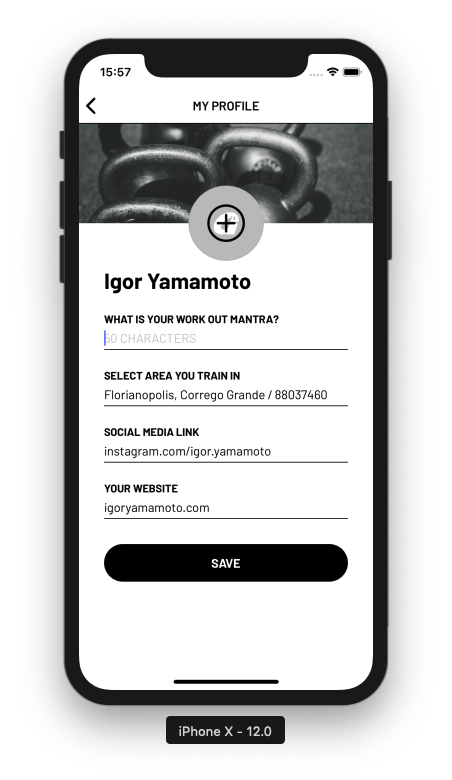
\includegraphics[width=\textwidth]{pfc/figuras/tr-register-profile-1.png}
        \caption{Registro das informações gerais do treinador}
        \label{fig:register-tr-profile-info}
    \end{subfigure}
    ~
	\begin{subfigure}[b]{0.3\textwidth}
        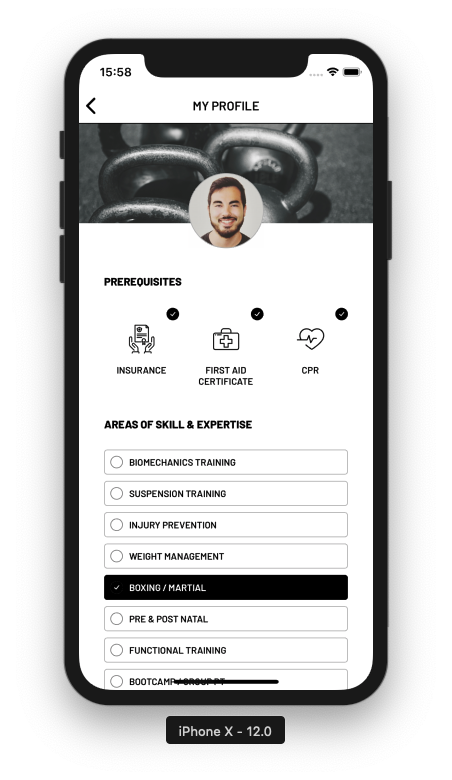
\includegraphics[width=\textwidth]{pfc/figuras/tr-register-profile-2.png}
        \caption{Registro das habilidades e especialidades}
        \label{fig:register-tr-skills}
    \end{subfigure}
    ~
    \begin{subfigure}[b]{0.3\textwidth}
        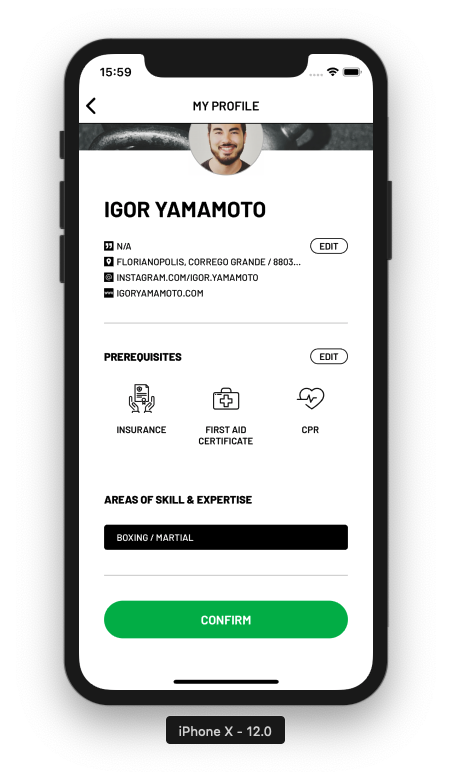
\includegraphics[width=\textwidth]{pfc/figuras/tr-register-profile-3.png}
        \caption{Confirmação do registro de perfil}
        \label{fig:register-tr-profile-confirmation}
    \end{subfigure}
    ~
    \caption{Fluxo de cadastro de perfil de treinador}
    \label{fig:register-tr-profile}
\end{figure}

% *******************
% Interface academias
% *******************
\section{Interface para Academias}
Nesta secção, é apresentada a interface de uso dos usuários que cadastraram um estabelecimento na plataforma. As principais funcionalidades implementadas para a versão piloto do aplicativo são abordadas: dashboard com dados semanais de uso da academia, calendário de sessões agendadas e configuração de agenda semanal para locação, perfil da academia.

Na interface para as academias o usuário tem a opção de navegar por cinco telas principais, selecionadas a partir da barra de navegação na parte inferior do aplicativo (Figura \ref{fig:gym-tabbar}). Da esquerda para a direita, as opções de navegação são: dashboard da academia; treinadores com sessões agendadas (não implementado para o piloto); calendário de sessões agendadas; central de notificações (não implementado para o piloto); perfil do estabelecimento.

Todos os dados que aparecem nas telas são provenientes de chamadas de API feitas ao back-end da aplicação. De acordo com o endpoint acessado, o back-end realiza o acesso ao banco de dados remoto da aplicação, efetua cálculos e aplica as lógicas de negócio se necessário. Em seguida, o mesmo envia a resposta à requisição. A chamada geralmente é feita no momento em que os componentes da tela são carregados ou imediatamente antes de serem renderizados. Mais detalhes desta integração são discutidos no próximo capítulo.

\begin{figure}[H]
    \centering
    
\includegraphics{pfc/figuras/gym-tabbar.png}
    \caption{Barra de navegação da interface para academias}
    \label{fig:gym-tabbar}
\end{figure}


\subsection{Dashboard da Academia}
A tela de dashboard da academia (Figura \ref{fig:gym-dashboard}) apresenta dados de uso e de receita semanais do estabelecimento. Os seguintes dados da semana corrente e anterior são apresentados no painel: receita total, número total de agendamentos, número total de treinadores, número total de hora agendadas por treinadores.

\begin{figure}[H]
    \centering
    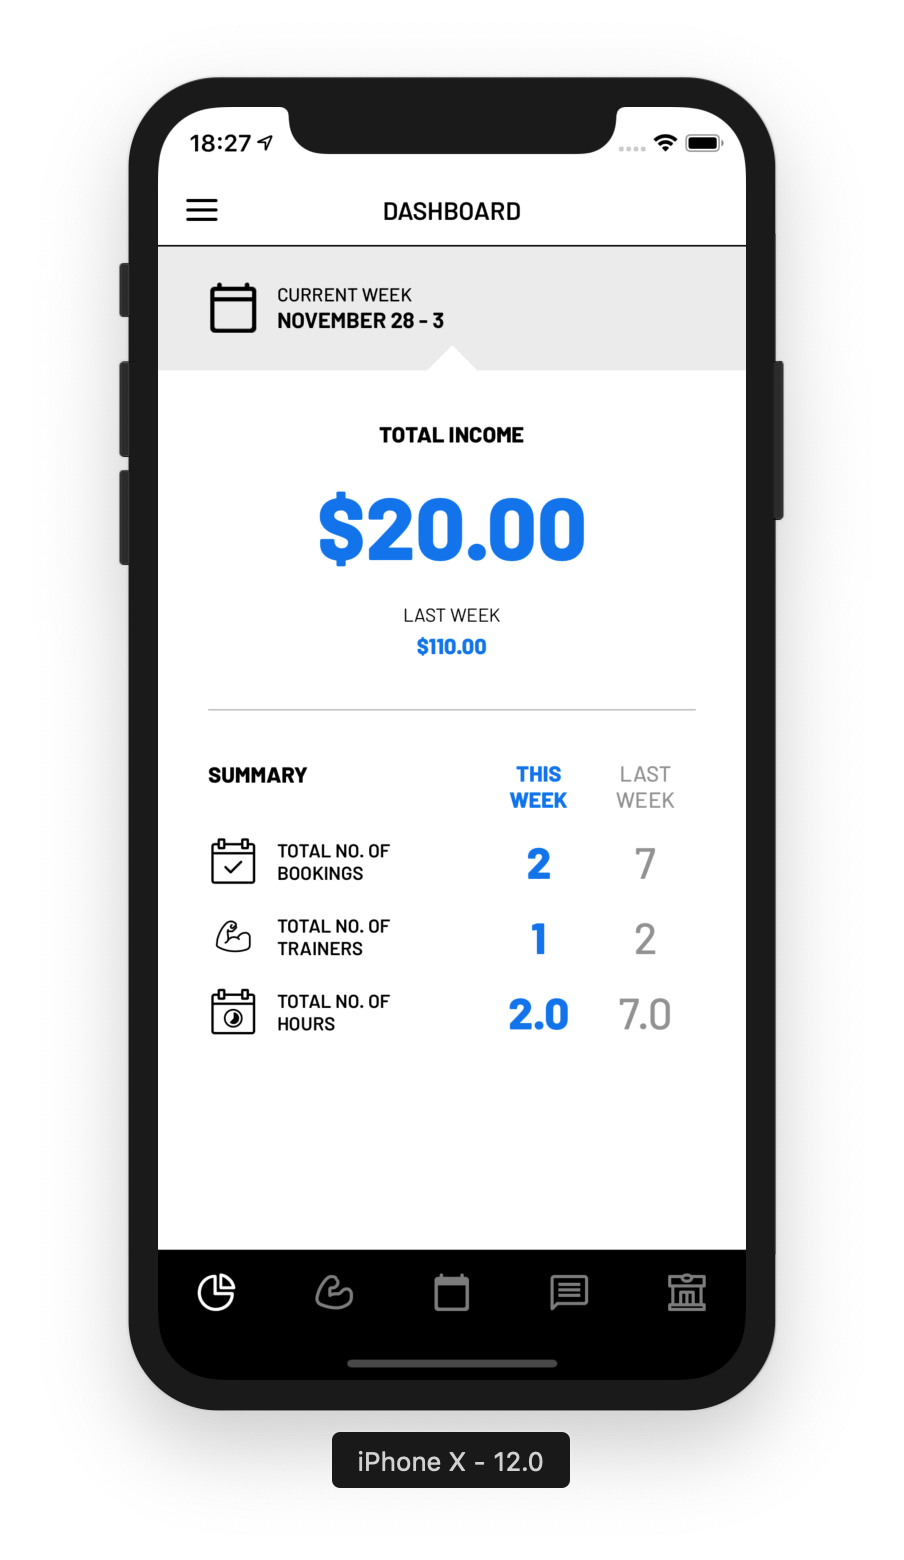
\includegraphics[width=0.4\textwidth]{pfc/figuras/gym-dashboard.png}
    \caption{Tela de dashboard da academia}
    \label{fig:gym-dashboard}
\end{figure}

\subsection{Agenda Semanal para Locação}
Ao acessar pela primeira vez a interface das academias, o usuário é direcionado para uma tela (ver Figura \ref{fig:gym-block-onboard}) onde são passadas informações de como funciona a agenda de blocos de horários semanais para locação da academia. A aplicação permite que as academias cadastrem blocos de horários fixos para cada dia da semana. Cada bloco contém a informação de taxa cobrada por hora, máximo número de pessoas permitidas e limites inferior e superior de horário para sessões. A partir destes blocos, os treinadores podem agendar sessões dentro dos mesmos (selecionando o número de clientes que eles vão levar, respeitando o limite máximo, e escolhendo o horário de início e término de uma sessão dentro dos limites de horário do bloco).

A Figura \ref{fig:gym-add-block} ilustra a tela de adição de um bloco semanal. As seguintes informações devem ser passadas: horários limites de início e término das sessões de treino, seleção de dias da semana nos quais o bloco será aplicado (ou seja, se academia quer disponibilizar blocos idênticos para diferentes dias da semana, ela utiliza esta opção), máximo número de pessoas permitidas dentro do bloco em um dado momento e, por último, taxa por hora cobrada dos treinadores.

Após a adição de blocos, os mesmos são exibidos na agenda (Figura \ref{fig:gym-block}) na posição correspondente aos limites de horário do bloco (blocos não podem ter limites de horários sobrepostos). Ao clicar no botão "Edit", o usuário pode editar as informações do bloco previamente fornecidas.

\begin{figure}[H]
	\centering
    \begin{subfigure}[b]{0.3\textwidth}
        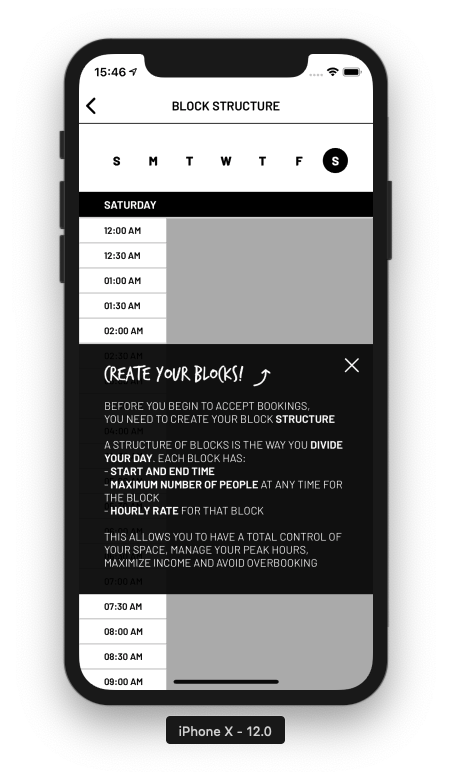
\includegraphics[width=\textwidth]{pfc/figuras/gym-block-structure-onboard.png}
        \caption{Instruções da agenda semanal}
        \label{fig:gym-block-onboard}
    \end{subfigure}
    ~
	\begin{subfigure}[b]{0.3\textwidth}
        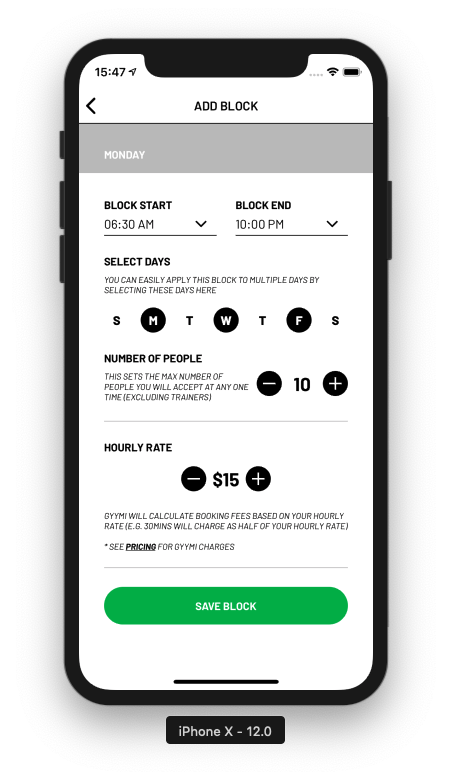
\includegraphics[width=\textwidth]{pfc/figuras/gym-add-block.png}
        \caption{Adição de novo bloco semanal}
        \label{fig:gym-add-block}
    \end{subfigure}
    ~
    \begin{subfigure}[b]{0.3\textwidth}
        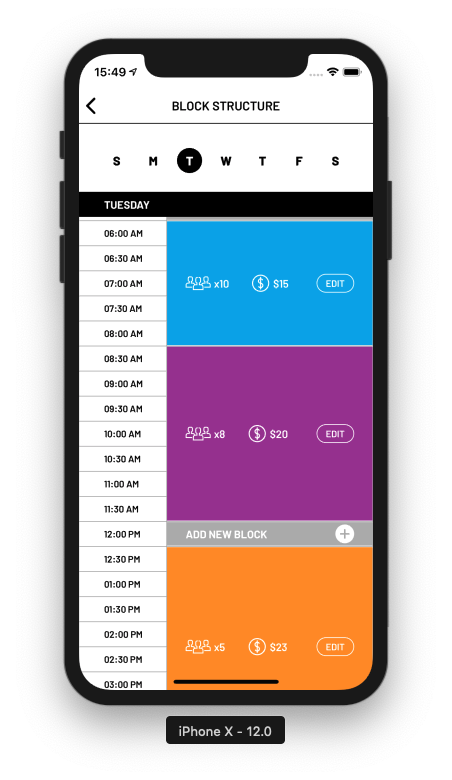
\includegraphics[width=\textwidth]{pfc/figuras/gym-block-structure.png}
        \caption{Agenda semanal da academia populada}
        \label{fig:gym-block}
    \end{subfigure}
    ~
    \caption{Fluxo de criação de blocos de horários para agenda semanal das academias}
    \label{fig:}
\end{figure}

\subsection{Calendário de Sessões Agendadas}
A tela de calendário de sessões agendadas (Figura \ref{fig:gym-calendar}) mostra informações gerais de agendamento de sessões filtradas por data. Na parte superior da interface, é possível selecionar a data em que se deseja obter informações através de um calendário. Em seguida dados da data selecionada são exibidos (número de treinadores e clientes do dia e receita esperada para o dia). Por fim, uma agenda com os blocos do dia é apresentada, com a indicação de quantos treinadores e seus respectivos clientes marcaram sessões de treino em cada bloco.

Ao clicar o botão "View details" localizado em cada um dos blocos, a tela de detalhes de agendamentos (Figura \ref{fig:gym-booking-detail}) é exibida. Nesta tela, todas as sessões agendadas no bloco selecionado são listadas. Cada sessão é detalhada em um card, contendo o nome completo do treinador, horários de início e término da sessão, total a pagar e número de clientes que o mesmo vai levar ao estabelecimento.

\begin{figure}[H]
	\centering
    \begin{subfigure}[b]{0.4\textwidth}
        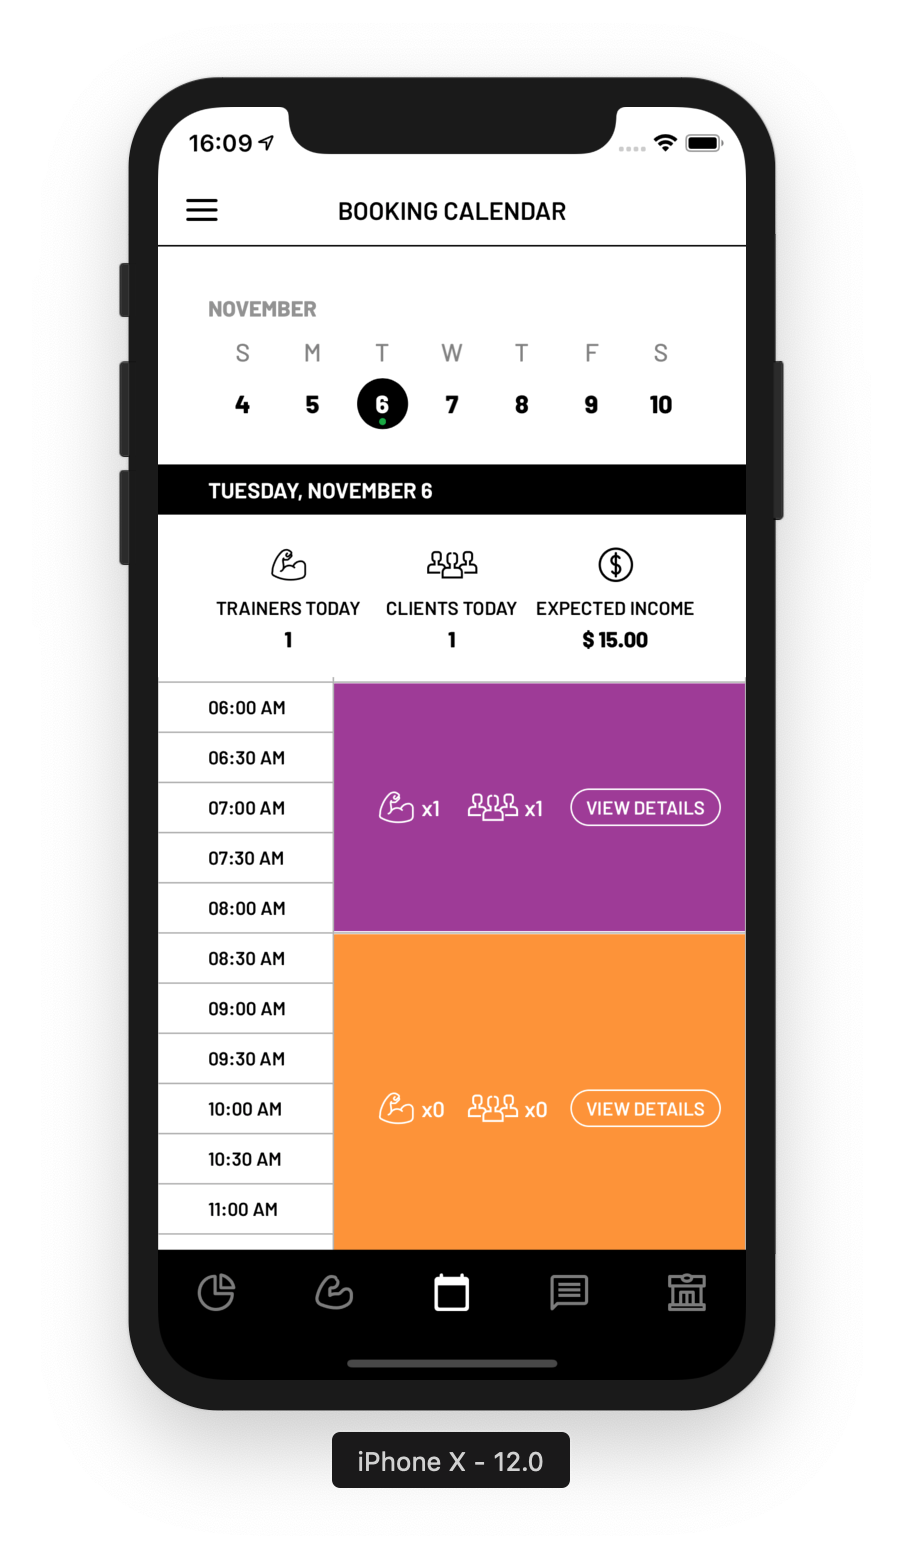
\includegraphics[width=\textwidth]{pfc/figuras/gym-booking-calendar.png}
        \caption{Calendário de sessões}
        \label{fig:gym-booking-calendar}
    \end{subfigure}
    ~
	\begin{subfigure}[b]{0.4\textwidth}
        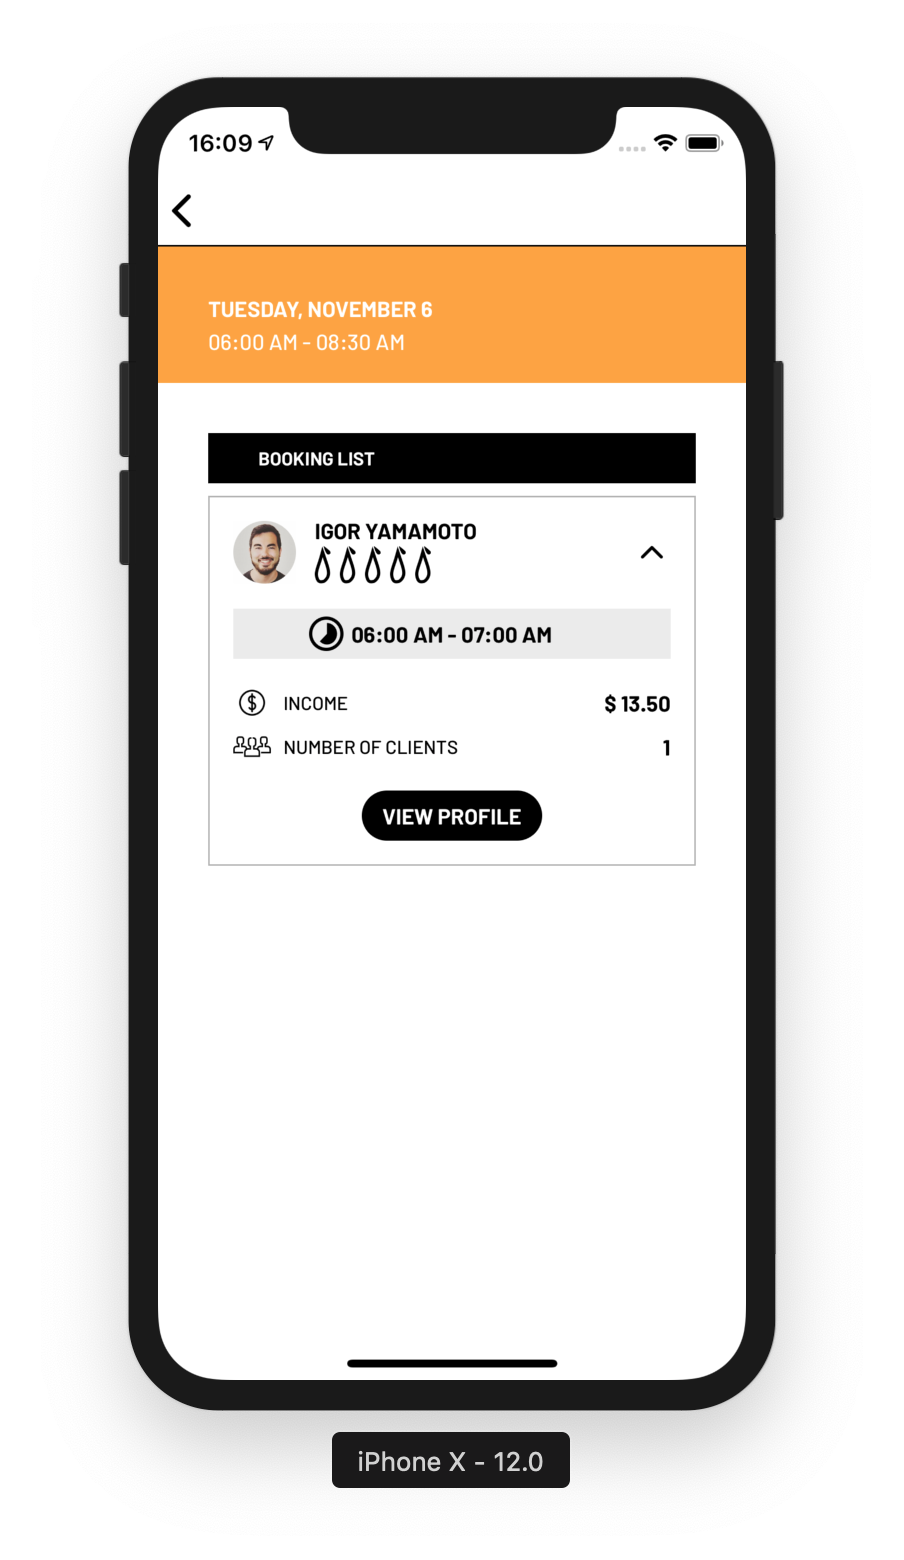
\includegraphics[width=\textwidth]{pfc/figuras/gym-booking-detail.png}
        \caption{Detalhes da sessão}
        \label{fig:gym-booking-detail}
    \end{subfigure}
    ~
    \caption{Telas do calendário de sessões agendadas na academia}
    \label{fig:gym-calendar}
\end{figure}

\subsection{Perfil do Estabelecimento}
A tela de perfil da academia além de exibir todos os dados passados pelo usuário no momento do cadastro, também mostra um indicador da nota do estabelecimento (de $1$ a $5$, calculada como sendo a média das avaliações de sessões de treino) e um mapa com a marcação da localização da academia. A interface permite que o usuário clique no botão "Edit" para que possa realizar edições no perfil previamente preenchido no momento do cadastro.

\begin{figure}[H]
    \centering
    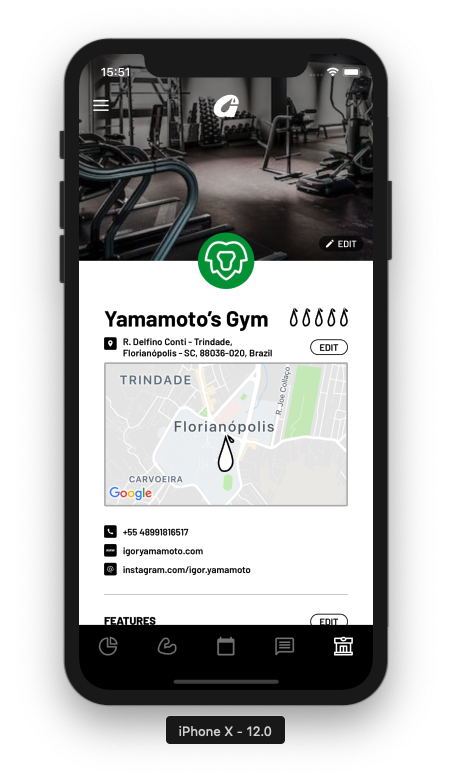
\includegraphics[width=0.4\textwidth]{pfc/figuras/gym-profile.png}
    \caption{Tela de perfil da academia}
    \label{fig:gym-profile}
\end{figure}

% *********************
% Interface treinadores
% *********************
\section{Interface para Treinadores}



\subsection{Busca por Academias}

\subsection{Agendamento de Sessão}

\subsection{Calendário de Sessões Agendadas}

\subsection{Perfil do Treinador}